\documentclass{thesis}
\usepackage[utf8]{inputenc} % 
\usepackage[T5]{fontenc} % Font Vietnamese
\usepackage{graphicx} % Figure
\usepackage{float} % Set position figure or table
\usepackage{mathptmx} % select font Times New Roman
\usepackage{geometry} % Set parameters paper
\usepackage{xcolor}
\usepackage[fontsize=13pt]{scrextend} % set font size = 13pt
\usepackage{indentfirst} % Indent first line
\usepackage{amsmath}
\usepackage{tikz}
\usetikzlibrary{shapes.geometric, arrows}
\usetikzlibrary{positioning}
\usepackage{pgf-umlsd}

%% FLOWCHART CONFIGURATION
% flowchart config
\tikzstyle{startstop} = [rectangle, rounded corners, 
minimum width=3cm, 
minimum height=1cm,
text centered, 
draw=black, 
fill=red!30]

\tikzstyle{io} = [trapezium, 
trapezium stretches=true, % A later addition
trapezium left angle=70, 
trapezium right angle=110, 
minimum width=3cm, 
minimum height=1cm, text centered, 
draw=black, fill=blue!30]

\tikzstyle{process} = [rectangle, 
minimum width=4cm, 
minimum height=1cm, 
text centered, 
text width=4cm, 
draw=black, 
fill=orange!30]

\tikzstyle{decision} = [diamond, 
minimum width=3cm, 
minimum height=1cm, 
text centered, 
draw=black, 
fill=green!30]

\tikzstyle{arrow} = [thick,->,>=stealth]
% end flowchar config

% block diagram config
\tikzstyle{block} = [draw, fill=blue!20, rectangle, 
    minimum height=3em, minimum width=6em]
\tikzstyle{sum} = [draw, fill=blue!20, circle, node distance=1cm]
\tikzstyle{input} = [coordinate]
\tikzstyle{output} = [coordinate]
\tikzstyle{pinstyle} = [pin edge={to-,thin,black}]

%% START DOCUMENT
\begin{document}

% COVER PAGE
%% CREATE COVER PAGE

\begin{center}
    \vspace{12pt} % line spacing
    \vspace{0.5cm}
    
% INSERT LOGO
\begin{figure}[H]
    \centering
    
\includegraphics[width=2cm,height=3cm]{figure/logoBK.png}
\end{figure}

% THESIS TYPE
\vspace{48pt}
        \fontsize{25pt}{0pt}\selectfont{} \textbf{GRADUATION THESIS}
\vspace{24pt}

 % THESIS TITTLE
        \textbf{\fontsize{17pt}{0pt}\selectfont{} WAREHOUSE MANAGEMENT SYSTEM}

        \textbf{\fontsize{17pt}{0pt}\selectfont{} DESIGN FOR SMART WAREHOUSE}
    \vspace{48pt}

% STUDENT NAME
        \fontsize{14pt}{0pt}\selectfont{} \textbf{NGUYỄN PHÚ QUYỀN}
    \vspace{3pt}

% STUDENT EMAIL    
        \fontsize{14pt}{0pt}\selectfont{} quyen.np192246@sis.hust.edu.vn
    \vspace{12pt} % line spacing

% STUDENT MAJOR
        \fontsize{14pt}{0pt}\selectfont{} \textbf{Advanced Program of Control and Automation Engineering}  
\end{center}
    \vspace{48pt}

% INFORMATION: SUPERVISOR NAME, STUDENT NAME,...
\begin{table}[H]
    \centering
        \begin{tabular}{l l c}
            \textbf{Instructor:}    &  M.Sc. Đinh Thị Lan Anh \vspace{6pt} &  \\ 
            &\vspace{3pt} & \fontsize{10pt}{0pt}\selectfont{} Instructor's signature \\
            \textbf{Department:} & Automation \vspace{3pt}\\ 
            \textbf{School:} & Electrical and Electronic Engineering
        \end{tabular}
\end{table}

% TIME
\begin{center}
    \vspace{48pt}
    \fontsize{14pt}{0pt}\selectfont{} Hanoi, 03/2023
\end{center}

% BLANK PAGE
% CREATE A NEW PAGE AND REMOVE PAGE NUMBER
\thispagestyle{empty}
    \newpage
        \clearpage
            \thispagestyle{empty}
                \cleardoublepage

% THESIS TASK
\input{relevant/task}
                
% THANKS
% THANKS
\section*{ACKNOWLEDGEMENT}
    \thispagestyle{empty}
    \indent
My heartfelt gratitude goes to Ms. Dinh Thi Lan Anh for her invaluable guidance and assistance. Her support was one of the most critical factors in helping me \linebreak overcome numerous obstacles along the way. Without her help and the favorable conditions she provided, I would not have been able to complete this project.

I would like to express my deep gratitude to all the teachers at the School of Electrical Engineering, as well as those from other schools, for imparting their knowledge to me over the past four years. The lessons I have learned during my time in university will serve as a compass, guiding me in the right direction for my future endeavors.

Although I have put forth my best, my abilities and knowledge regarding this matter are limited. Hence, errors are inevitable. Therefore, I would greatly appreciate your guidance and any additional suggestions you may have in order to improve this project.

Once again, I would like to express my sincerest gratitude for all the help and lessons that I have received.

\vspace{6pt}
    \hspace{7.5cm}Hanoi, date 28, month 03, year 2023
        
        \hspace{10cm} Student      % command '\hspace' used to line indents

\vspace{2cm}
    \hspace{9.25cm}\textbf{Nguyễn Phú Quyền} % change name

% BLANK PAGE
% CREATE A NEW PAGE AND REMOVE PAGE NUMBER
\thispagestyle{empty}
    \newpage
        \clearpage
            \thispagestyle{empty}
                \cleardoublepage

% SUMMARY
\section*{ABSTRACT}
    \thispagestyle{empty}
Vietnam's warehouse management systems have undergone significant changes over the years, driven by a combination of factors such as economic growth, \linebreak globalization, and technological advancements. With Vietnam rapidly transforming into a manufacturing and logistics hub for the region, there has been an increased demand for modern and efficient warehouses. As a result, warehouse management strategies have become a popular topic among economists, scientists, and engineers.

Tien Phong Plastic Joint Stock Company is one of the leading plastic \linebreak manufacturers in Vietnam, producing a wide range of plastic products for various industries. To manage their warehouse operations, it is essential to have a warehouse management system for their factories and warehouses.

The aim of this thesis is to first analyze the layout and system of Tien Phong's warehouse. Then, modeling and quantifying the value of the warehouse operations to make optimization and operation easier. Finally, proposing solutions and designing a standalone warehouse management system for Tien Phong Plastic Joint Stock \linebreak Company's warehouse.

%% TOC
\thispagestyle{empty}
    \cleardoublepage

 % CONTENT
\tableofcontents 
    \thispagestyle{empty}
        \newpage
            \thispagestyle{empty}
                \cleardoublepage

% LIST OF SYMBOLS AND ABBREVIATIONS
\pagenumbering{roman}   % Roman numbering: i, ii, iii, iv,...
\section*{LIST OF ACRONYMS}
    \phantomsection \addcontentsline{toc}{section}{\numberline{} LIST OF ACRONYMS}

% Create table
\begin{tabular}{ l l }
    \hspace{1cm} WMS & \hspace{2cm} Warehouse Management System    \\
    \hspace{1cm} TPP & \hspace{2cm} Tien Phong Plastic Joint Stock Company \\
    \hspace{1cm} RFID & \hspace{2cm} Radio Frequency Identification \\
    \hspace{1cm} SQL & \hspace{2cm} Structured Query Language \\
    \hspace{1cm} ABC  & \hspace{2cm} ABC Analysis \\
    \hspace{1cm} SKU  & \hspace{2cm} Stock Keeping Unit \\
\end{tabular}  
    \newpage

% LIST OF FIGURES
{\let\oldnumberline\numberline
    \renewcommand{\numberline}{Figure~\oldnumberline}
        \listoffigures}
            \phantomsection\addcontentsline{toc}{section}{\numberline{} LIST OF FIGURES}
\newpage

% LIST OF TABLES
{\let\oldnumberline\numberline
    \renewcommand{\numberline}{Table~\oldnumberline}
        \listoftables}
            \phantomsection\addcontentsline{toc}{section}{\numberline{} LIST OF TABLES}
\newpage

\pagenumbering{arabic} % numbering: 1,2,3,...

%---------------------------------------------------------%%
%% ----------CHAPTER 1-------------------%%
%---------------------------------------------------------%%
\section*{CHAPTER 1. INTRODUCTION} 
    \addcontentsline{toc}{section}{\numberline{}CHAPTER 1. INTRODUCTION}

\setcounter{section}{1} 
    \setcounter{subsection}{0}
        \setcounter{subsubsection}{0}
            \setcounter{paragraph}{0}
                \setcounter{figure}{0}
                    \setcounter{table}{0}
                        \setcounter{equation}{0}
%%--------------------------------------------------------
\subsection{Smart warehouse}

A warehouse is a large commercial building used for storage and distribution of goods. It typically contains rows of shelving or storage racks where products are stored until they are needed for shipping or other purposes. \cite{smith2019warehouse}

A smart warehouse, on the other hand, is a warehouse that uses advanced \linebreak technologies such as RFID tags to track inventory, autonomous robots or drones for material handling, and predictive analytics to forecast demand and optimize supply chain operations. Additionally, data analytics may be used to monitor and improve warehouse processes, as well as reduce waste. \cite{Abhijeet2019}

Overall, the goal of a smart warehouse is to create a highly efficient and \linebreak responsive supply chain that can quickly adapt to changing market demands and customer needs.

The main objectives of warehouse management activities can be listed as:
        \begin{itemize}
            \begin{itemize}
                \item Quality management.
                \item Quantity management.
                \item Space optimization.
                \item Resource optimization.
                \item Synchronization.
            \end{itemize}
        \end{itemize}

Managing plastic productions can be challenging due to the large number of categories and limited technology in Vietnamese companies. Most warehouse \linebreak management systems in Vietnam are manual, which is time-consuming and costly. Plastic products come in various sizes and shapes, requiring more storage space and higher expenses. Additionally, customer needs for plastic products are diverse and unstable, making warehouse management volatile, which creates problems for balancing customer satisfaction with storage costs. \cite{Duong2019}

To overcome these challenges, the implementation of a warehouse management system (WMS) is necessary. By automating warehouse operations, a WMS can improve inventory accuracy and reduce the costs associated with manual labor.

\subsection{Project objective}
The main objective of the project is to propose suitable solutions for the warehouse management system. To achieve this objective, several tasks need to be completed:
        \begin{itemize}
            \begin{itemize}
                \item  Analyze and evaluate the current layout and operations of warehouse \linebreak management activities.
                \item Determine the specifications of plastic products that need to be considered.
                \item Derived from the current warehouse a suitable system model.
                \item Suggesting improvements to enhance efficiency taking into account existing process.
                \item Develop a warehouse management system in accordance with the identified specifications and requirements.
            \end{itemize}
        \end{itemize}

\subsection{Thesis approach}

The approach to the topic follows the scientific process, ensuring objectivity and reliability. The process begins with an overview of research related to warehouse management to identify new trends. The current status of the chosen warehouse is then evaluated to determine its performance efficiency. Based on this data, an appropriate management method for the warehouse is selected and applied. After the development process, opportunities and benefits are considered for deploying the new system application to the current warehouse. Finally, the new warehouse management system is developed and tested.

Several techniques and methods were applied during the development of the new system. Theoretical research was conducted by reviewing domestic and international literature related to smart warehouse management systems. This helped identify key factors for the management system and successful experiences of typical enterprises and corporations. Theoretical research is an effective and scientific method to find information, identify research gaps, and provide a feasible implementation strategy for actual conditions.

After conducting theoretical research, appropriate designs for equipment and software were proposed based on the major requirements and analysis of the \linebreak warehouse's operations. As the complex requirements of a plastic warehouse cannot be met by existing management software options, it is decided that a suitable software will be develop according to the characteristics of the plastic industry. Two options were considered: web-based or traditional software on a computer. Both options have open sources and frameworks that support development, but a web-based application was chosen over software due to its ability to run directly on many devices without requiring installation on every computer.

The last technique employed involves analyzing data gathered from associations, organizations, and units to assess the level of conformity of enterprises with the requirements of the WMS. The gathered information is analyzed based on parameters such as the number and size of the enterprise, its business field, management capacity, infrastructure, technology level, as well as production and business status to determine their suitability for the WMS.

\newpage

%---------------------------------------------------------%%
%% ----------CHAPTER 2-------------------%%
%---------------------------------------------------------%%
\section*{CHAPTER 2. OVERVIEW}
    \addcontentsline{toc}{section}{\numberline{} CHAPTER 2. OVERVIEW}

\setcounter{section}{2}
    \setcounter{subsection}{0}
        \setcounter{subsubsection}{0}
            \setcounter{paragraph}{0}
                \setcounter{figure}{0}
                    \setcounter{table}{0}
                        \setcounter{equation}{0}
%---------------------------------------------------------%
\subsection{Tien Phong warehouse}

\subsubsection{Tien Phong Plastic Joint Stock Company}

Tien Phong Plastic Joint Stock Company is a leading producer and distributor of plastic products in Vietnam \cite{vietnam_report_2021}. The company was established in 1975 and has since become one of Vietnam's largest plastic manufacturers, offering a wide range of products, including plastic pipes, fittings, and packaging materials.

\subsubsection{Tien Phong warehouse}

\paragraph{Layout}\mbox{}

Based on the information in the appendix (see {\autoref{fig:premiese}} and \autoref{fig:design}), it appears that there is currently no shelf or rack system in the warehouse. This can make it difficult to locate and retrieve items quickly, which increases order fulfillment times and negatively impacts overall warehouse operations. While a shelf or rack system is not strictly necessary, it can greatly enhance the efficiency and effectiveness of the warehouse. \cite{rack_system_smart_warehouse}

In order to develop a suitable system and design solution in the later chapters, a custom rack system is recommended. An orthographic projection of each location with a rack system suitable for the carton box (size 40x60x40) has been designed.

    \begin{figure}[!ht]
        \centering
        
\includegraphics[scale=0.75]{figure/location.png}
        \caption{Orthographic projection of one location}
        \label{fig:location}
    \end{figure}

As shown in \autoref{fig:location}, four shelves with 25 slots each (5x5) have been added. Additionally, there are 2 aisles (0.66 meters) between the shelves at each location.

Based on the recalculations, the storage capacity of each unit is as follows:
\begin{itemize}
    \begin{itemize}
        \item Slot: 0.13 cubic meter;
        \item Shelf: 3.33 cubic meter;
        \item Location: 13.31 cubic meter;
        \item All: 2395.01 cubic meter.
    \end{itemize}
\end{itemize}

It is important to consider orthographic projections of sections in addition to the overall warehouse design. By examining the sections of the warehouse, it is possible to gain a more detailed understanding of how the space can be utilized most effectively.

    \begin{figure}[!ht]
        \centering
        
\includegraphics[scale=0.7]{figure/warehouse1.png}
        \caption{Top projection of sections}
        \label{fig:top}
    \end{figure}

In total, TPP's warehouse include: 
\begin{itemize}
    \begin{itemize}
        \item 3 floors;
        \item 8 sections;
        \item 180 locations;
        \item 720 shelfs;
        \item 18000 slots.
    \end{itemize}
\end{itemize}    

    \begin{figure}[!ht]
        \centering
        
\includegraphics[scale=0.7]{figure/warehouse2.png}
        \caption{Front projection of sections}
        \label{fig:front}
    \end{figure}

    \begin{figure}[!ht]
        \centering
        
\includegraphics[scale=0.7]{figure/warehouse3.png}
        \caption{Side projections of sections}
        \label{fig:side}
    \end{figure}

\paragraph{Process}\mbox{}

As shown from the report of TPP warehouse (\autoref{fig:manuallabour} and \ref{fig:recinf}), it appears that the current management processes are mostly manual labor, which is both time-consuming and costly. In the span of 10 months, a total of 1,008,832 products (\autoref{fig:rep2019}) were found to be sitting idly in storage in only 4 of the 8 sections. Moreover, the price range of each product varies significantly, from a few thousand to several million Vietnamese dong. The cost of labor and time required to handle such a significant backlog of products is substantial, and it highlights the need for a more efficient and streamlined management process.

Based on analysis of the statistics and research data, It is estimate that with the implementation of the new rack system, each slot will change its contents approximately ten times on average per year. This estimate takes into account factors such as the size and type of items being stored, as well as the expected frequency of inventory turnover. \cite{tienphongplastic}

\subsection{Warehouse management system}

Warehouse management refers to the process of organizing, controlling, and managing the operations of a warehouse. This includes the receipt, storage, and distribution of goods and materials. Warehouse management aims to optimize the use of space, labor, and equipment to ensure that products are stored, tracked, and delivered efficiently. \cite{Kumar2019}

Warehouse management systems (WMS) are software applications that help manage the operations of a warehouse. They provide real-time information about inventory levels, order processing, and shipping. A WMS typically uses technologies such as barcode scanners, RFID tags, and automated material handling equipment to optimize warehouse operations.  \cite{Kumar2019}

The use of a WMS can provide several benefits, including:
\begin{itemize}
    \begin{itemize}
        \item Improved inventory accuracy: A WMS provides real-time information about inventory levels, reducing the risk of overstocking or understocking.
        \item Increased efficiency: By automating warehouse operations, a WMS can reduce the time and labor required to manage inventory, orders, and shipping.
        \item Enhanced customer service: A WMS can help ensure that products are delivered to customers on time and in good condition, improving customer satisfaction.
        \item Cost savings: By optimizing warehouse operations, a WMS can reduce labor costs, minimize inventory holding costs, and reduce shipping expenses.
    \end{itemize}
\end{itemize}

\subsection{Management Process}

\subsubsection{Receiving and put-away}

    \begin{figure}[!ht]
        \centering
        
\includegraphics[width=13cm,height=11cm]{figure/processes.png}
        \caption{Receiving and put-away processes}
        \label{fig:wmprocess}
    \end{figure}
    
Although warehouses differ in terms of size, type, function, ownership and location some fundamental processes remain (\autoref{fig:wmprocess}).

\paragraph{Receiving}\mbox{}

Receiving, goods-in or in-handling is a crucial process within the warehouse. 
Ensuring that the correct product has been received in the right quantity and in the right condition at the right time is one of the mainstays of the warehouse operation. These elements are often termed supplier compliance.

\paragraph{In-handling}\mbox{}

One Of the main challenges for a warehouse manager is to match labour hours with work content. Handling a product the least amount of time possible (labour touch points) leads to reduced labour hours and as a consequence, reduced cost. \cite{richards2014warehouse}

Depending on the operation, labour can be the single biggest cost within a warehouse. It can be between 48 and 60 percents Of the total warehouse cost depending on the amount Of automation utilized. It is also the most difficult
cost to control. \cite{richards2014warehouse}

In-handling makes up approximately 20 per cent of the total direct labour
cost within a retail warehouse. \cite{richards2014warehouse}

\paragraph{Put-away}\mbox{}

Many of today's WMSs allocate product locations in advance and instruct the operator as to where to place the goods. This can be directly to the despatch area if the product is to be cross docked as discussed above, to the pick face as a form of replenishment or to a reserve or bulk-storage location.

In order for this system to work effectively, a great deal of information needs to be programmed into the system. This includes the following:
\begin{itemize}
    \begin{itemize}
        \item size, weight and height of palletized goods;
        \item results of an ABC analysis or slotting, where fast-moving goods are
        \item placed closest to the despatch area;
        \item current order data;
        \item family product groups;
        \item actual sales combinations;
        \item current status of pick face for each product.
    \end{itemize}
\end{itemize}

\subsubsection{Order picking}

    \begin{figure}[!ht]
        \centering
        
\includegraphics[width=16cm,height=9cm]{figure/picking.png}
        \caption{Picking relationships}
        \label{fig:pickingrelationships}
    \end{figure}

Order picking is the most costly activity within today's warehouses. Not only is it labour intensive, but it is challenging to automate, can be difficult to plan, is prone to error and crucially has a direct impact on customer service (see \autoref{fig:pickingrelationships}). Typical errors include omitting items from the order, sending the wrong item and sending the wrong number of items.

\paragraph{Warehouse pick area layout}\mbox{}

Having produced a comprehensive profile of the products and orders, layout is next to be considered.

    \begin{figure}[!ht]
        \centering
        
\includegraphics[width=16cm,height=13cm]{figure/layout.png}
        \caption{Sample warehouse layout based on ABC classification}
        \label{fig:layout}
    \end{figure}
    
\autoref{fig:layout} depicts a very basic layout that has used an ABC analysis based on the frequency of pick-face visits. The next step is to minimize the amount of travel through the warehouse when picking an order. \cite{vandenberg2013optimizing}

    \begin{figure}[!ht]
        \centering
        
\includegraphics[width=15cm,height=12cm]{figure/sequence.png}
        \caption{Picking route}
        \label{fig:sequence}
    \end{figure} 

The route followed by the picker when assembling the order needs to take into account the following: \cite{vandenberg2013optimizing}
\begin{itemize}
    \begin{itemize}
        \item The pick instruction will have each pick sequenced as per the most effective route beginning at the front of the racking nearest the despatch bays.
        \item Heaviest items are picked first.
        \item The picker should be able to pick from both sides when moving up and down the aisles. See \autoref{fig:sequence} below. In this example the aisles are numbered, not the rows of racking which means that the picker can move from side to side as opposed to travelling up the length of the racking and back down the other side.
        \item Shortcuts are programmed into the system to minimize travel. For example, a break in a long length of racking (as shown in {fig:layout}) enables the picker to shorten the travel distance but allows the storage of reserve product above the pathway.
        \item The picker ends up as close to the despatch area as possible. If the picker is not operating in real time the picker may need to return  to the start point to pick up a new assignment. This is not ideal.
        \item Multiple pick locations for the most popular items need to be set up to avoid congestion at the pick bays.
    \end{itemize}
\end{itemize}

\subsection{Storage strategies}

The organization of warehouses, inputs, and outputs is influenced by what is known as "storage strategies". While these strategies are not primarily focused on what and where items are stored, they do prioritize the structural arrangement of these elements. The most common ones are: FIFO, LIFO, FEFO, HIFO, ...

\subsubsection{FIFO}

FIFO stands for "First-In, First-Out" and is an inventory management method that assumes that the first items received into an inventory are the first to be sold or used. This means that the oldest inventory items are used or sold first, while the newer items are used or sold later. FIFO is commonly used for products that have a limited shelf life or are perishable, such as food or medicine, to ensure that the older items are used first and do not expire. It can also help businesses manage product obsolescence by ensuring that older products are sold or used before newer ones.
   
\subsubsection{LIFO}

LIFO stands for "Last-In, First-Out" and is an inventory management method that assumes that the last items received into an inventory are the first to be sold or used. This means that the newest inventory items are used or sold first, while the older items are used or sold later. LIFO is commonly used for products that have a long shelf life and are not likely to expire or spoil, such as furniture or electronics. It can also help businesses manage rising costs by using the most recently purchased and typically more expensive inventory items first, which can result in lower taxes and higher profits. However, LIFO may not be suitable for businesses that need to track inventory based on expiration dates or other specific characteristics.
    
\subsubsection{FEFO}

FEFO stands for "First-Expired, First-Out" and is an inventory management method that assumes that the first products that will expire are the first to be sold or used. This method is commonly used for products that have a limited shelf life or are perishable, such as food, medicine, or cosmetics. By using the FEFO method, businesses can ensure that they use or sell the products that are closest to their expiration dates first, reducing the risk of spoilage or waste.

\newpage

%---------------------------------------------------------%%
%% ----------CHAPTER 3-------------------%%
%---------------------------------------------------------%%
\section*{CHAPTER 3. MODELING}
    \addcontentsline{toc}{section}{\numberline{}CHAPTER 3. MODELING}
    
\setcounter{section}{3}
    \setcounter{subsection}{0}
        \setcounter{subsubsection}{0}
            \setcounter{paragraph}{0}
                \setcounter{figure}{0}
                    \setcounter{table}{0}
                        \setcounter{equation}{0}
%%-------------------------------------------------------%%
% --------------------------------------------------------%
%---------------------------------------------------------%
\subsection{System model}

\subsubsection{Coordinate}

To accurately locate the position of a slot, it is essential to establish a coordinate system. The coordinate system provides a framework for identifying the exact location of each slot within the warehouse space. By using a coordinate system, it is possible to implement a more efficient and organized storage system that can help streamline warehouse operations and optimize inventory management:
    \begin{equation}\label{eq:coordinate}
        X(i) = \text{ [Floor][Section][Location][Shelf][Column][Row]}
    \end{equation}

    \begin{figure}[!ht]
        \centering
        
\includegraphics[scale=0.45]{figure/sample1.png}
        \caption{A slot in section 8, location A}
        \label{fig:sample1}
    \end{figure}

    \begin{figure}[!ht]
        \centering
        
\includegraphics[scale=0.45]{figure/sample2.png}
        \caption{A slot in section 3, location 4}
        \label{fig:sample2}
    \end{figure}

The coordinate slot range from 11111 to 38D455 is established with limits and exception (as shown in table \ref{tab:coordinate}). These limits will provide a clear framework for locating and organizing items within the warehouse, which will help to improve efficiency and productivity.

    \begin{table}[H]
        \centering
        \caption{Coordinates}
        \begin{tabularx}{1\textwidth}{
            | >{\centering}a%\arraybackslash}y
            | >{\centering\arraybackslash}y
            | >{\centering\arraybackslash}y
            | >{\centering\arraybackslash}a|
            }
                \hline
            \bfseries  Type   
            &\bfseries Minimum  
            &\bfseries Maximum 
            & \bfseries Exception \\\hline
             Floor  & 1  & 3  &  \\\hline
             Section  & 1  & 8  &  \\\hline
             Location  & 1  & 7  & A,B,C,D (Section 8) \\\hline
             Shelf  & 1  & 4  &  \\\hline
             Column  & 1  & 5  &  \\\hline
             Row  & 1  & 5  &  \\\hline
        \end{tabularx}
        \label{tab:coordinate}
    \end{table}

\subsubsection{Layout}

\paragraph{Slot}\mbox{}

The following properties of both the slot and the item stored in the slot should be taken into consideration.

    Slot coordinate:
    \begin{equation}\label{eq:slot coordinate}
        X_s(i) = \text{ [Floor][Section][Location][Shelf][Column][Row]}
    \end{equation}

    Preferred item identification code to be stored:
    \begin{equation}\label{eq:pref IC}
        I_p(i) = \text{ [item code]}
    \end{equation}

    Denote if the slot is empty or not: 
    \begin{equation}\label{eq:empty}
        E_s(i) =  
        \begin{cases}
            1, & \text{ if there is item stored} \\
            0, & \text{ if there the slot is empty} \\
        \end{cases}
    \end{equation}
    
    Stored item identification code: 
    \begin{equation}\label{eq:stored item IC}
        I_s(i) =  
        \begin{cases}
            \text{ [item code]}, & \text{if  } E_s(i) = 1 \\
            0, & \text{if  } E_s(i) = 0 \\
        \end{cases}
    \end{equation}
        
    Stored carrier (carton box) identification code: 
    \begin{equation}\label{eq:storedcarrierIC}
        I_{sc}(i) =  
        \begin{cases}
            \text{ [carrier code]}, & \text{if  } E_s(i) = 1 \\
            0, & \text{if  } E_s(i) = 0 \\
        \end{cases}
    \end{equation}
    
    The timestamp when the item is stored:
    \begin{equation}\label{eq:stored timestamp}
        T_s(i) = \text{ [received timestamp]}
    \end{equation}
    
    Denote if the product is already reserved for order: 
    \begin{equation}\label{eq:reserved}
        R_d(i) =
        \begin{cases}
            1, & \text{ if stored item is reserved} \\
            0, & \text{ if stored item is not reserved} \\
        \end{cases}
    \end{equation}
        
    Order identification code: 
    \begin{equation}\label{eq:order IC}
        I_d(i) =  
        \begin{cases}
            \text{ [order code]}, & \text{if  } R_d(i) = 1 \\
            \text{ [null]}, & \text{if  } R_d(i) = 0 \\
        \end{cases}
    \end{equation}
    
    The estimate despatch timestamp, day, month, year: \quad 
    ${T_d(i), D_d(i), M_d(i), Y_d(i)}$

    Item shelf age at the date of calculation: 
    \begin{equation}\label{slot shelf age}
        T_a(i) = \text{ [now timestamp]} - T_s(i)
    \end{equation}

\paragraph{Column}\mbox{}
    
    Column coordinate:
    \begin{equation}\label{eq:column coordinate}
        X_c(i) = \text{ [Floor][Section][Location][Shelf][Column]}
    \end{equation}
    
    Preferred item identification code to be stored:
    \begin{equation}\label{eq:prefered column IC}
        I_c(i) = \text{ [item code]}
    \end{equation}

    Column storage capacity by slot: 
    \begin{equation}\label{eq:column capacity}
        C_c(i) = 5 - \sum_{j=1}^{5} E_s(f[X_c(i),j])
    \end{equation}

    Column age by the oldest product shelf age: 
    \begin{equation}\label{eq:column age}
        T_c(i) = max[T_a(f[X_c(i)])]
    \end{equation}

\paragraph{Shelf}\mbox{}

    Shelf coordinate:
    \begin{equation}\label{eq:shelf coordinate}
        X_f(i) = \text{ [Floor][Section][Location][Shelf]}
    \end{equation}
    
    Shelf storage capacity by slot: 
    \begin{equation}\label{eq:shelf capacity}
        C_f(i) = \sum_{j=1}^{5} C_c(f[X_f(i),j])
    \end{equation}

\paragraph{Location}\mbox{}

    Location coordinate:
    \begin{equation}\label{eq:location coordinate}
        X_n(i) = \text{ [Floor][Section][Location]}
    \end{equation}
    
    Location storage capacity by slot: 
    \begin{equation}\label{eq:location capacity}
        C_n(i) = \sum_{j=1}^{4} C_f(f[X_n(i),j])
    \end{equation}

\subsubsection{Parameters}

It is important to ensure that the warehouse does not operate at full capacity at all times, as this can lead to potential issues in the event of an emergency. Therefore, we recommend designating specific areas within the warehouse as emergency storage locations. In this case, we suggest assigning locations A, B, C, and D as emergency storage areas, along with the slots within those areas. By designating these specific locations as emergency storage, we can ensure that there is always enough space available to accommodate unexpected inventory or other urgent needs. This will help to ensure that the warehouse can operate safely and efficiently, even in the event of an emergency.

    Total slots: \quad
    ${ S_{t} = 18000 }$

    Available slots for allocate: \quad
    ${S_{a} = 16800}$

    Emergency slots: \quad
    ${ S_{e} = 1200 = \frac{1}{15} S_{t} }$

    Total number of product: \quad
    ${ W = 434 }$

\subsubsection{Product}

    Item code: \quad
    ${ I(i) }$
    
    Number of product per carrier: \quad
    ${ U(i) }$
    
    Price of each product: \quad
    ${ P_e(i) }$

    Price of each carrier:
    \begin{equation}\label{eq:price}
        P(i) = P_e(i) \times U(i)
    \end{equation}
    
    Cost of each product: \quad
    ${ A_e(i) }$
    
    Cost of each carrier:
    \begin{equation}\label{eq:cost}
        A(i) = A_e(i) \times U(i)
    \end{equation}
    
    Product profit per carrier:
    \begin{equation}\label{eq:profit}
        B(i) = P(i) - A(i)
    \end{equation}

\paragraph{Statistic}\mbox{}

    Total number of stored carrier of the product in the warehouse: 
    \begin{equation}\label{eq:Qs}
        Q_s(i) = \sum_{j=1}^{S_t}
        \begin{cases}
            E_s(j), & \text{if  } I(i) = I_s(j) \\
            0, & \text{if  } I(i) \neq I_s(j) \\
        \end{cases}
    \end{equation}

    Total number of reserved carrier of the product in the warehouse:
    \begin{equation}\label{eq:Qd}
        Q_d(i) = \sum_{j=1}^{S_t}
        \begin{cases}
            R_d(j), & \text{if  } I(i) = I_s(j) \\
            0, & \text{if  } I(i) \neq I_s(j) \\
        \end{cases}
    \end{equation}
    
    Total number of available carrier of the product in the warehouse: 
    \begin{equation}\label{eq:Qa}
        Q_a(i) = Q_s(i) - Q_d(i)
    \end{equation}

    Oldest available carrier coordinate:
    \begin{equation}\label{eq:Xo}
        X_o(i) = X(j), \quad \text{ if }
        \begin{cases}
            I(i) = I_s(j) \\
            R_d(j) = 0 \\
            T_a(j) = max[T_a(f[I(i)])] \\
        \end{cases}
    \end{equation}

    Newest stored carrier coordinate:
    \begin{equation}\label{eq:Xt}
        X_t(i) = X(j), \quad \text{ if }
        \begin{cases}
            I(i) = I_s(j) \\
            R_d(j) = 0 \\
            T_s(j) = min[T_s(f[I(i)])] \\
        \end{cases}
    \end{equation}

\paragraph{Record}\mbox{}

    Number of days each year: \quad
    ${ Z_{Y_d(j)} }$ (days) \quad <example: ${Z_{2022} = 365}$ days)>

    Total number of days since recorded: \quad
    \begin{equation}\label{eq:Zr}
        Z_r = \sum Z_{Y_d(j)} \text{ (days)}
    \end{equation}

    Number of orders product appear on each year: \quad
    ${ O_{Y_d(j)}(i) }$ (orders)

    Total number of orders involved since recorded:
    \begin{equation}\label{eq:Or}
        O_r(i) = \sum O_{Y_d(j)}(i) \text{ (orders)}
    \end{equation}

    Number of days product appear on order each year: \quad
    ${ D_{Y_d(j)}(i) }$ (days)

    Total number of days involved since recorded: \quad
    \begin{equation}\label{eq:Dr}
        D_r(i) = \sum D_{Y_d(j)}(i) \text{ (days)}
    \end{equation}

    The number of days involved will not exceed the number of orders involved:
    \begin{equation}\label{eq:leqdayorderannual}
        D_{Y_d(j)}(i) \leq O_{Y_d(j)}(i)
    \end{equation}
    \begin{equation}\label{eq:leqdayorderall}
        D_r(i) \leq O_r(i)
    \end{equation}

    Number of carrier despatched each year: \quad
    ${ Q_{Y_d(i)}(i) }$ (carriers)

    Total number of carrier despatched recorded: \quad
    \begin{equation}\label{eq:Qr}
        Q_r(i) = \sum Q_{Y_d(j)}(i) \text{ (carriers)}
    \end{equation}

    It is important to note that:
    \begin{equation}\label{eq:leqQYd}
        \sum_{i=1}^{W} Q_{Y_d(j)}(i) \leq S_t \times Z_{Y_d(j)}
    \end{equation}
    \begin{equation}\label{eq:leqQr}
        \sum_{i=1}^{W}Q_{r(j)}(i) \leq S_t \times Z_{r}
    \end{equation}

    The frequency, or ratio of appearance of the product:
    \begin{equation}\label{eq:FYd}
        F_{Y_d(j)}(i) = \frac{D_{Y_d(j)}(i)}{Z_{Y_d(j)}}
    \end{equation}
    \begin{equation}\label{eq:Fr}
        F_r(i) = \frac{D_r(i)}{Z_r}
    \end{equation}

    The average flow of product:
    \begin{equation}\label{eq:GYd}
        G_{Y_d(j)}(i) = \frac{Q_{Y_d(j)}(i)}{O_{Y_d(j)}(i)} \text{ (carrier per order)}
    \end{equation}
    \begin{equation}\label{eq:Gr}
        G_r(i) = \frac{Q_r(i)}{O_r(i)} \text{ (carrier per order)}
    \end{equation}
    \begin{equation}\label{eq:gYd}
        g_{Y_d(j)}(i) = \frac{Q_{Y_d(j)}(i)}{D_{Y_d(j)}(i)} \text{ (carrier per day)}
    \end{equation}
    \begin{equation}\label{eq:gr}
        g_r(i) = \frac{Q_r(i)}{D_r(i)} \text{ (carrier per day)}
    \end{equation}
    
    Combined with equation \eqref{eq:leqdayorderannual} and \eqref{eq:leqdayorderall}:
    \begin{equation}\label{eq:geqgYd}
        g_{Y_d(j)}(i) \geq G_{Y_d(j)}(i)
    \end{equation}
    \begin{equation}\label{eq:geqgr}
        g_{r(j)}(i) \geq G_{r(j)}(i)
    \end{equation}

    The average slot demand of product:
    \begin{equation}\label{eq:HYd}
        H_{Y_d(j)}(i) = \frac{Q_{Y_d(j)}(i)}{Z_{Y_d(j)}}
        \text{ (slot per day)}
    \end{equation}
    \begin{equation}\label{eq:Hr}
        H_r(i) = \frac{Q_r(i)}{Z_r}
        \text{ (slot per day)}
    \end{equation}

\subsection{Control objective}

\subsubsection{Space allocation}

    Total average slot demand of all products:
    \begin{equation}\label{eq:VYd}
        V_{Y_d(j)} = \sum_{k=1}^{W} H_{Y_d(j)}(k) 
        = \sum_{k=1}^{W} \frac{Q_{Y_d(j)}(i)}{Z_{Y_d(j)}}
        \leq S_t
    \end{equation}
    
    \begin{equation}\label{eq:Vr}
        V_r = \sum_{k=1}^{W} H_r(k) 
        = \sum_{k=1}^{W} \frac{Q_{r}(i)}{Z_{r}}
        \leq S_t
    \end{equation}

    Total stored slot in the warehouse at the current date:
    \begin{equation}\label{eq:Vs}
        V_s = \sum_{j=1}^{S_a} E_s(j) \leq S_a
    \end{equation}

    Total empty slot in the warehouse at the current date:
    \begin{equation}\label{eq:Ve}
        V_e = S_a - V_s
    \end{equation}

    Total emergency slot in use at the current date:
    \begin{equation}\label{eq:Vemc}
        V_{emc} = \sum E_s(f[X_{emc}]) \leq S_e
    \end{equation}

    Total empty column in the warehouse at the current date:
    \begin{equation}\label{eq:Ke}
        K_e = \sum_{i=1}^{3360}
        \begin{cases}
            1, & \text{if } C_c(i) = 5 \\
            0, & \text{if } C_c(i) < 5 \\
        \end{cases}
        \quad \text{ also } K_e \leq \frac{V_e}{5}
    \end{equation}

\paragraph{First cycle}\mbox{}

    In case ${ V_s = 0 }$
            
    All time value of each product:
    \begin{equation}\label{eq:Nri}
        N_r(i) = Q_r(i) \times B(i)
    \end{equation}

    All time value of all products:
    \begin{equation}\label{eq:Nr}
        N_r = \sum_{i=1}^{W} N_r(i) 
    \end{equation}

    Percentage of all time value for each product:
    \begin{equation}\label{eq:Lri}
        L_r(i) = \frac{N_r(i)}{N_r}
    \end{equation}

    In accord to the annual percentage ${ L_r(i) }$ and frequency ${ F_r(i) }$ of each product, which is sorted from high to low. Applying ABC analysis method, the number of columns allocate to each product can be calculated.
    \begin{equation}\label{eq:K}
        K(i) = 
        \begin{cases}
            \frac{max[g_r(i),H_r(i)]}{5}, & 
            \text{case A} \\
            \frac{max[G_r(i),H_r(i)]}{5}, & 
            \text{case B} \\
            \frac{min[G_r(i),H_r(i)]}{5}, & 
            \text{case C} \\
        \end{cases}
    \end{equation}

    As long as the following condition is sastified:
    \begin{equation}\label{eq:conditionK}
        \sum_{i=1}^{W} K(i) \leq \frac{S_a}{5}
    \end{equation}

    Further elaborate with equation \eqref{eq:Gr} and \eqref{eq:Vr} in case C of equation \eqref{eq:K}:
    \begin{equation}\label{eq:elaborate first cycle}
        \sum_{i=1}^{W} min[G_r(i),H_r(i)] \leq 
        \sum_{k=1}^{W} H_{Y_r}(i)
        \leq S_t
    \end{equation}

    Also statistic report in 2019 (appendix A) show that:
    \begin{equation}\label{eq:report 2019}
        \sum_{i=1}^{W} U(i) \times Q_{2019}(i) = 75982216, 
        \text{ with } U_{avg} \approx 458
    \end{equation}

    Hence average slot demand of all products in 2019:
    \begin{equation}\label{eq:sample 2019}
        V_{2019} = \sum_{i=1}^{W} \frac{Q_{2019}(i)}{Z_{2019}} \approx 165900 
        \approx \frac{1}{39,6} \times S_t
    \end{equation}

\paragraph{Annual cycle}\mbox{}

    Previous year:
    \begin{equation}\label{eq:Yp}
        Y_p = 2022 \text{ (sample)}
    \end{equation}

    Annual value of each product:
    \begin{equation}\label{eq:NYpi}
        N_{Y_p}(i) = Q_{Y_p}(i) \times B(i)
    \end{equation}

    Annual value of previous year:
    \begin{equation}\label{eq:NYp}
        N_{Y_p} = \sum_{i=1}^{W} N_{Y_p }(i) 
    \end{equation}

    Percentage of annual value for each product:
    \begin{equation}\label{eq:LYpi}
        L_{Y_p}(i) = \frac{N_{Y_p }(i)}{ N_{Y_p }}
    \end{equation}

   In accord to the annual percentage ${ L_{Y_p}(i) }$ and frequency ${ F_{Y_p}(i) }$ of each product, which is sorted from high to low. Applying ABC analysis method, the number of columns allocate to each product can be calculated.
    \begin{equation}\label{eq:Ka}
        K_a(i) = 
        \begin{cases}
            K_e \times \frac{max[g_{Y_p}(i),H_{Y_p}(i)]}{S_a}, & 
            \text{case A} \\
            K_e \times \frac{max[G_{Y_p}(i),H_{Y_p}(i)]}{S_a}, & 
            \text{case B} \\
            K_e \times \frac{min[G_{Y_p}(i),H_{Y_p}(i)]}{S_a}, & 
            \text{case C} \\
        \end{cases}
    \end{equation}
    
    As long as the following condition is sastified:
    \begin{equation}\label{eq:ConditionKa}
        \sum_{i=1}^{W} K_a(i) \leq K_e
    \end{equation}

It is worth noting that the annual cycle can be adjusted to a quarterly or monthly cycle to allow for more flexible space allocation. By adjusting the cycle to a shorter timeframe, it becomes easier to adjust warehouse operations based on changes in inventory needs and other factors. This can help to optimize space allocation and improve overall warehouse efficiency.

\subsubsection{Receiving and put-away}

Although TPP plastic products have a lifespan of about 50 years, it is still important to have a storage strategy in place to prevent products from sitting on the shelf for too long. Therefore, a FIFO (first in, first out) strategy has been chosen to ensure that older products are used or sold before newer ones.

Based on the FIFO strategy, the following variables are to be considered when the system receives a new carrier: product identification code ${ I }$ and the corresponding product newest stored coordinate ${ X_t }$.

    Find youngest column with suitable capacity (there is empty slot within):
    \begin{equation}\label{eq:rap find X}
        X = 
        \begin{cases}
            f[X_c(f[X_t])], & \text{if } C_c(f[X_t]) > 0 \\
            f[X_c(j)], & \text{if }
            \begin{cases}
                C_c(f[X_t]) = 0 \\
                T_c(j) = min[T_c(f[I])] \\
                C_c(j) > 0 \\
            \end{cases}
        \end{cases}
    \end{equation}

In case there are multiple empty columns as well as full columns that have been designated for a specific product, it is recommend to select the empty column that is closest to the full ones:
    \begin{equation}\label{eq:empty find X}
        X = f[X_c(j)], \quad
            \begin{cases}
                C_c(f[I]) = 0 \\
                C_c(f'[I]) = 5 \\
                |j-f[I]| \text{ is minimum}
            \end{cases}
    \end{equation}

\subsubsection{Order fulfillment}

There are two scenarios: either the total available product carrier ${ Q_a(i) }$ is \linebreak sufficient to fulfill the order, or it is insufficient.

\paragraph{Sufficient}\mbox{}

When considering the age column, columns ${ X_c(i) }$ are selected from the oldest to the youngest <${ T_c(i) }$>. In each column, carriers ${ X(i) }$ are selected using the same principle <${ T_a(i) }$>.

    Hence, there is no emergency request send to the factory:
    \begin{equation}\label{eq:no emc}
        \text{\emph{EMC(i)}} =  0
    \end{equation}

\paragraph{Insufficient}\mbox{}

Place a replenishment request for the emergency locations. Carriers in here should be placed order by order, with priority given to the first order to be picked.
    \begin{equation}\label{eq:emc}
        \text{\emph{EMC(i)}} =  
        \text{\emph{order numbers (i)}} - Q_a(i)
    \end{equation}

    Provided that the following condition is met:
    \begin{equation}\label{eq:sum emc}
        \sum EMC_{D_d} \leq \text{\emph{ factory capacity}}
    \end{equation}

\subsubsection{Daily replenishment}

To calculate the daily replenishment for the warehouse, both the factory capacity and emergency requests need to be taken into consideration.
    \begin{equation}\label{eq:drq}
        \text{\emph{daily replenishment quota}} = 
        \text{\emph{factory capacity}} - \sum EMC{D_d} 
    \end{equation}

Based on the product frequency from the previous year ${ F_{Y_d} }$, products should be picked in order of higher frequency, while ensuring that the total replenishment does not exceed the quota.
    \begin{equation}\label{eq:quota}
        \sum C_c(i) = \sum (5 \times K_a(i)) + \sum C_{c,prev}(i)
        \leq \text{\emph{ daily replenishment quota}}
    \end{equation}

\subsection{Control algorithm}

\subsubsection{Space allocation}\label{ca:space allocation}

In the control loop shown in \autoref{fig:Space allocation control loop}, the input is the serial number of the product, and the output is the number of columns assigned to the product. The controller uses the annual percentage and frequency of each product, applying the ABC analysis method with equation \eqref{eq:conditionK} and \eqref{eq:ConditionKa} to generate a control signal that determines the output. The output is calculated using equation \eqref{eq:K} and \eqref{eq:Ka}.

    Control loop for space allocation cycle:
    \begin{figure}[!ht]
        \centering
        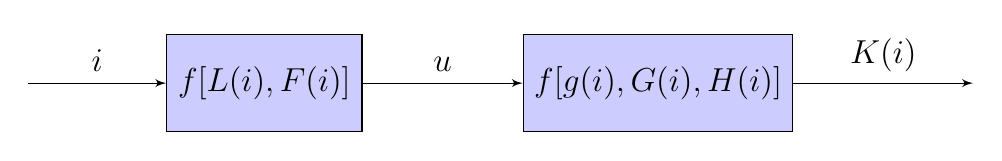
\begin{tikzpicture}[auto, node distance=2cm,>=latex']
            \node [input, name=input] 
            {};
            \node [block, right of=input, node distance=3cm] (controller) 
            {$f[L(i),F(i)]$};
            \node [block, right of=controller, node distance=5cm] (system) 
            {$f[g(i),G(i),H(i)]$};
            \node [output, right of=system, node distance=4cm] (output) 
            {};
            \draw [draw,->] (input) -- node 
            {$i$} (controller);
            \draw [->] (controller) -- node[name=u, above] 
            {$u$} (system);
            \draw [->] (system) -- node [name=y, above] 
            {$K(i)$}(output);
        \end{tikzpicture}
        \caption{Space allocation control loop block diagram}
        \label{fig:Space allocation control loop}
    \end{figure}

\subsubsection{Receiving and put-away}\label{ca:receiving and put-away}

Based on \autoref{fig:Receiving and put-away flowchart diagram}, the algorithm takes information about the new carrier as input and outputs the coordinate where the system will place it. The algorithm finds the most suitable slot that satisfies the FIFO strategy from the column that stores or is assigned to the same item.

A control algorithm for the receiving and put-away process was designed using equations \eqref{eq:rap find X} and \eqref{eq:empty find X}:
    \begin{figure}[!ht]
        \centering
        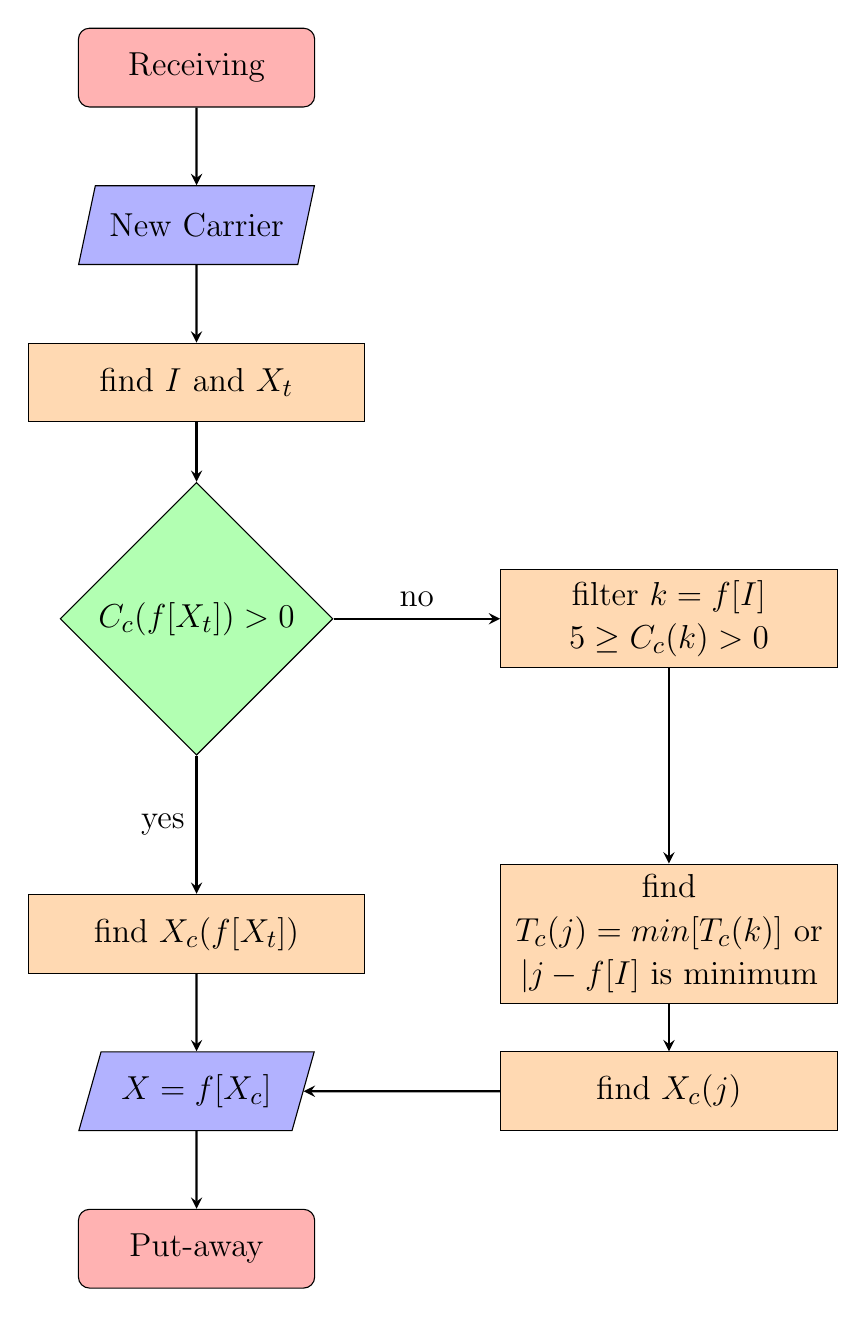
\begin{tikzpicture}[node distance=2cm]

        \node (start) [startstop] 
        {Receiving};
        \node (input) [io, below of = start] 
        {New Carrier};
        \node (proc1) [process, below of = input] 
        {find $I$ and ${X_t}$};
        \node (dec2) [decision, below of = proc1, yshift = -1cm] 
        {${C_c(f[X_t]) > 0}$};
    
        \node (proc2y) [process, below of = dec2, yshift = -2cm] 
        {find ${X_c(f[X_t])}$};
        \node (output) [io, below of=proc2y] 
        {${X=f[X_c]}$};
        \node (stop) [startstop, below of=output] 
        {Put-away};
                
        \node (proc2n) [process, right of = dec2, xshift = 4cm] 
        {filter ${k = f[I]}$ \\ ${5 \geq C_c(k) > 0}$};
        \node (proc3) [process, below of = proc2n, yshift = -2cm] 
        {find ${T_c(j) = min[T_c(k)]}$ or \linebreak ${|j-f[I]}$ is minimum};
        \node (proc4) [process, below of = proc3, yshift = 0cm] 
        {find ${X_c(j)}$};
        
        \draw [arrow] (start) -- (input);
        \draw [arrow] (input) -- (proc1);
        \draw [arrow] (proc1) -- (dec2);
        \draw [arrow] (dec2) -- node[anchor=east] {yes} (proc2y);
        \draw [arrow] (dec2) -- node[anchor=south] {no} (proc2n);
        \draw [arrow] (proc2y) -- (output);
        \draw [arrow] (output) -- (stop);
        
        \draw [arrow] (proc2n) -- (proc3);
        \draw [arrow] (proc3) -- (proc4);
        \draw [arrow] (proc4) -- (output);
        
        \end{tikzpicture}
        \caption{Receiving and put-away flowchart diagram}
        \label{fig:Receiving and put-away flowchart diagram}
    \end{figure}

\subsubsection{Order fulfillment}\label{ca:order fulfillment}

Based on the flowchart diagram for order fulfillment shown in \autoref{fig:Order fulfillment flowchart diagram}, the algorithm takes the product identification code from a new order as its input and outputs the locations where the system will pick the products. The algorithm finds the most suitable slot that satisfies the FIFO strategy and requests more products from the factory in cases where there are insufficient numbers.

A control algorithm for order fulfillment process is designed based on equations \eqref{eq:no emc}, \eqref{eq:emc}, and \eqref{eq:sum emc}:
    \begin{figure}[!ht]
        \centering
        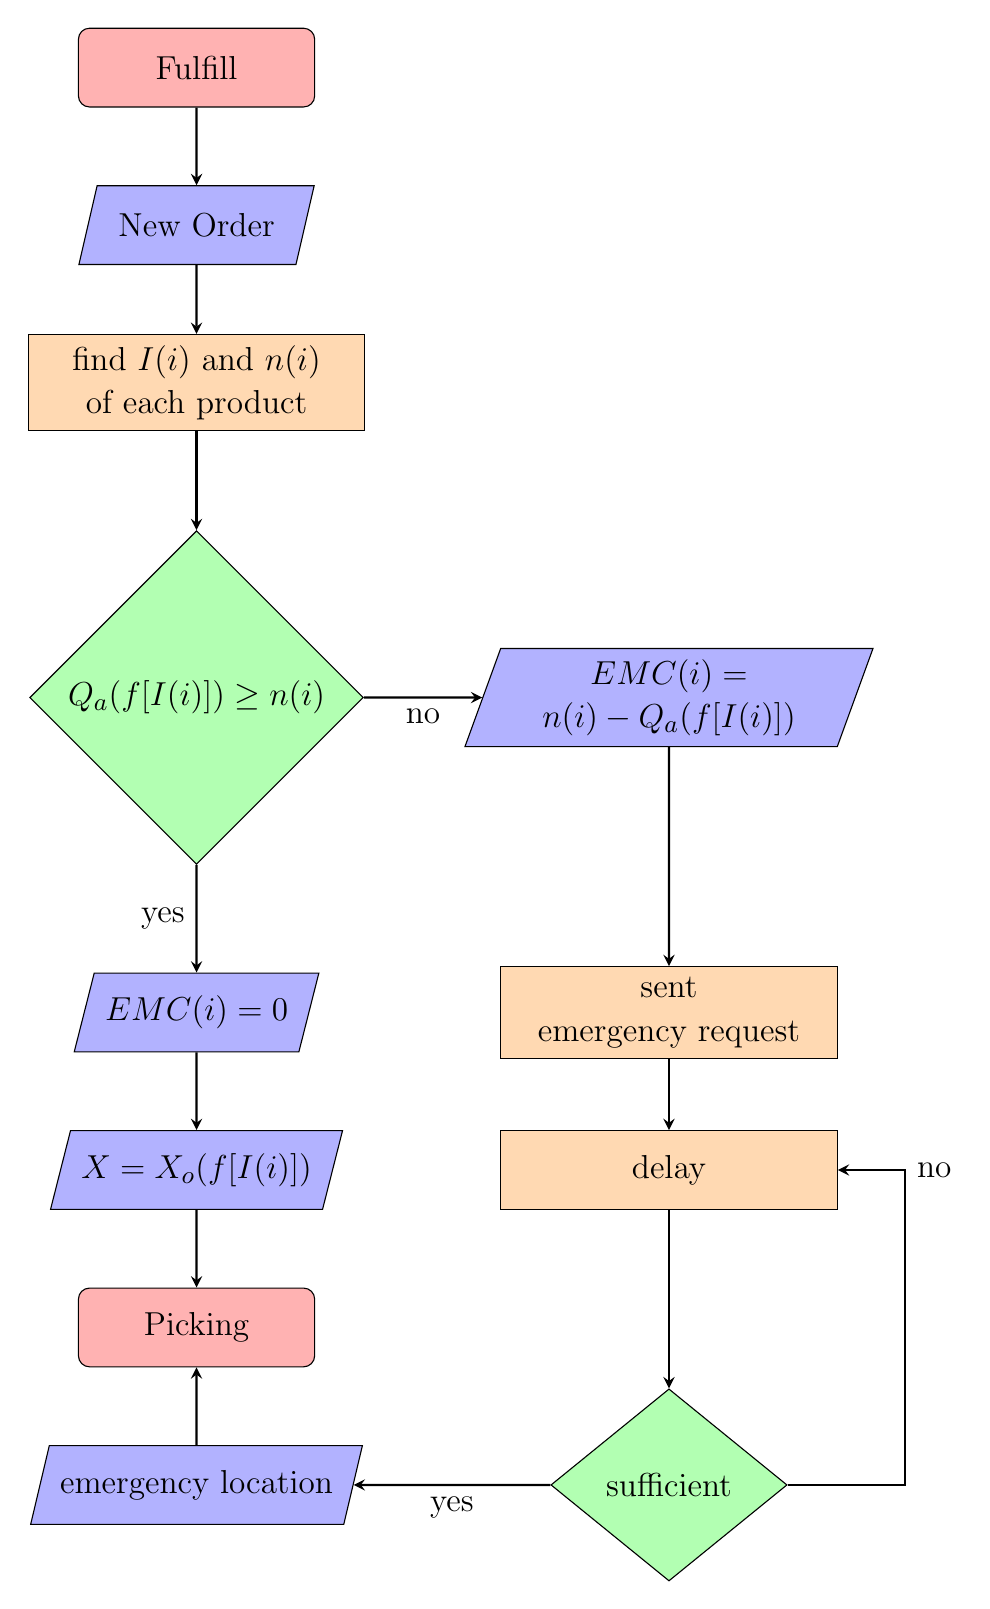
\begin{tikzpicture}[node distance=2cm]

        \node (start) [startstop] 
        {Fulfill};
        \node (input) [io, below of = start] 
        {New Order};
        \node (proc1) [process, below of = input] 
        {find $I(i)$ and $n(i)$ of each product};
        \node (dec2) [decision, below of = proc1, yshift = -2cm] 
        {${Q_a(f[I(i)]) \geq n(i)}$};
    
        \node (proc2y) [io, below of = dec2, yshift = -2cm] 
        {${EMC(i) = 0}$};
        \node (output) [io, below of=proc2y] 
        {${X=X_o(f[I(i)])}$};
        \node (stop) [startstop, below of=output] 
        {Picking};
                
        \node (proc2n) [io, right of=dec2, xshift=4cm, text width=4cm, align=center]
        {${EMC(i) = }$ \linebreak ${n(i) - Q_a(f[I(i)])}$};
        \node (proc3) [process, below of = proc2n, yshift = -2cm] 
        {sent \\ emergency request};
        \node (proc4) [process, below of = proc3, yshift = 0cm] 
        {delay };
        \node (dec3) [decision, below of = proc4, yshift = -2cm]
        {sufficient};
        \node (emc) [io, left of = dec3, xshift = -4cm]
        {emergency location};
        
        \draw [arrow] (start) -- (input);
        \draw [arrow] (input) -- (proc1);
        \draw [arrow] (proc1) -- (dec2);
        \draw [arrow] (dec2) -- node[anchor=east] 
        {yes} (proc2y);
        \draw [arrow] (dec2) -- node[anchor=north] 
        {no} (proc2n);
        \draw [arrow] (proc2y) -- (output);
        \draw [arrow] (output) -- (stop);

        \draw [arrow] (proc2n) -- (proc3);
        \draw [arrow] (proc3) -- (proc4);
        \draw [arrow] (proc4) -- (dec3);

        \draw [arrow] (dec3) -- node[anchor=north] 
        {yes} (emc);
        \draw [arrow] (dec3) -- ++(3cm,0) |- node[anchor=west] 
        {no} (proc4);
        \draw [arrow] (emc) -- (stop);
        
        \end{tikzpicture}
        \caption{Order fulfillment flowchart diagram}
        \label{fig:Order fulfillment flowchart diagram}
    \end{figure}

\subsubsection{Daily replenishment}\label{ca:replenishment}

In the control loop depicted in \autoref{fig:Replenishment control loop}, the input, or set point, is the total available slots for allocation. The feedback signal is the total number of stored slots (excluding emergency slots), which is calculated using equation \eqref{eq:Vs}. The output is the daily replenishment request sent to the factory. The disturbance is the emergency request. The error signal is the total number of empty slots (excluding emergency slots), calculated using equation \eqref{eq:Ve}. The actuating signal is the storage capacity of columns, calculated using equation \eqref{eq:column capacity}. The controller uses the product frequency to prioritize which product to replenish first.

    Replenishment control loop:
    \begin{figure}[!ht]
        \centering
        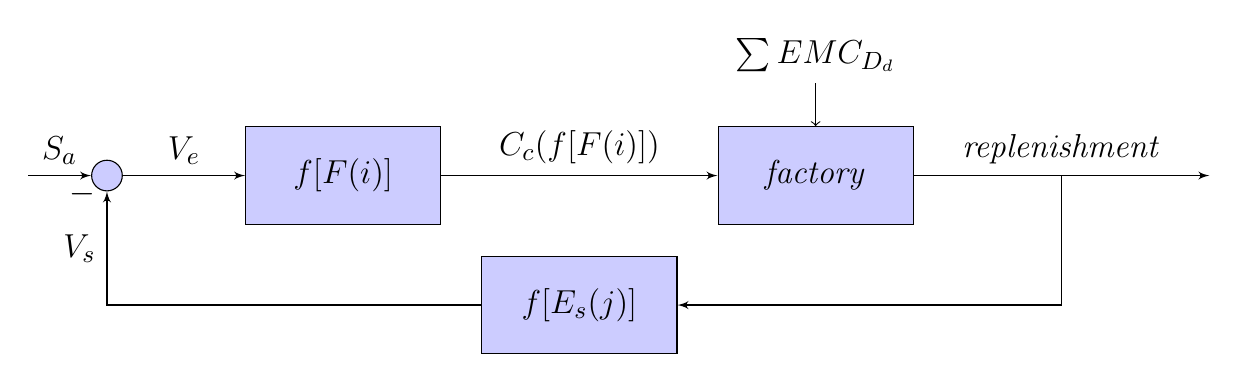
\begin{tikzpicture}[auto, node distance=2cm,>=latex']
            \node [input, name=input] 
            {};
            \node [sum, right of=input, node distance=1cm] (sum) 
            {};
            \node [block, right of=sum, node distance=3cm] (controller) 
            {$f[F(i)]$};
            \node [block, right of=controller, 
            pin={[pinstyle]above:$ \sum EMC_{D_d} $},
                node distance=6cm] (system) 
            {\emph{factory}};
            \draw [->] (controller) -- node[name=u, above] 
            {$C_c(f[F(i)])$} (system);
            \node [output, right of=system, node distance=5cm] (output) 
            {};
            \node [block, below of=u] (measurements) 
            {$f[E_s(j)]$};
            \draw [draw,->] (input) -- node 
            {$S_a$} (sum);
            \draw [->] (sum) -- node 
            {$V_e$} (controller);
            \draw [->] (system) -- node [name=y, above] 
            {\emph{replenishment}}(output);
            \draw [->] (y) |- (measurements);
            \draw [->] (measurements) -| node[pos=0.99] 
            {$-$} 
                node [near end] 
            {$V_s$} (sum);
        \end{tikzpicture}
        \caption{Replenishment control loop block diagram}
        \label{fig:Replenishment control loop}
    \end{figure}

\newpage

%---------------------------------------------------------%%
%% ----------CHAPTER 4-------------------%%
%---------------------------------------------------------%%
\section*{CHAPTER 4. DESIGN}
    \addcontentsline{toc}{section}{\numberline{} CHAPTER 4. DESIGN}
    
\setcounter{section}{4}
    \setcounter{subsection}{0}
        \setcounter{subsubsection}{0}
            \setcounter{paragraph}{0}
                \setcounter{figure}{0}
                    \setcounter{table}{0}
                        \setcounter{equation}{0}
%--------------------------------------------------------%
\subsection{System architecture}
A n-tier architecture is well-suited for a WMS due to its scalability, maintainability, security, and flexibility. It allows you to scale different parts of the system independently, make it easier to maintain and update the different layers, improve the security of the system, and give you more flexibility to choose different technologies or frameworks for each layer. \cite{wang2012ntier}
    \begin{figure}[!ht]
        \centering
        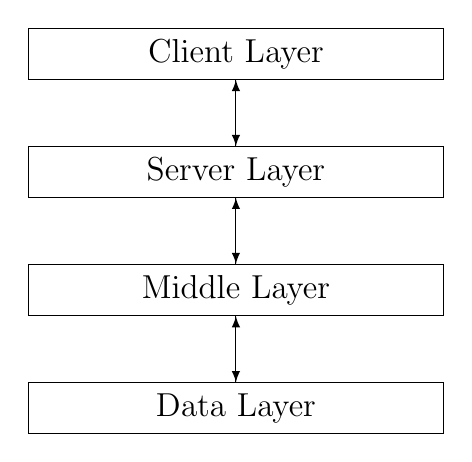
\begin{tikzpicture}[node distance=1.5cm]
            \node (client) [draw, text width=5cm, align=center] 
            {Client Layer};
            \node (server) [draw, text width=5cm, align=center, below of=client] 
            {Server Layer};
            \node (middle) [draw, text width=5cm, align=center, below of=server] 
            {Middle Layer};
            \node (data) [draw, text width=5cm, align=center, below of=middle] 
            {Data Layer};
        
            \draw [-latex] (client) -- (server);
            \draw [-latex] (server) -- (middle);
            \draw [-latex] (middle) -- (data);
            
            \draw [-latex] (server) -- (client);
            \draw [-latex] (middle) -- (server);
            \draw [-latex] (data) -- (middle);
        \end{tikzpicture}
        \caption{4-tier architecture}
        \label{fig:4-tier architecture}
    \end{figure}

\subsection{System flow}

\subsubsection{User login}

    \begin{figure}[!ht]
        \centering
        \resizebox{1\textwidth}{!}{
        \begin{sequencediagram}
            \newinst[2]{client}{Client Layer}
            \newinst[2]{server}{Server Layer}
            \newinst[2]{middle}{Middle Layer}
            \newinst[2]{data}{Data Layer}
                
            \begin{sdblock}{User login}
            {}
                \begin{call}
                    {client}{account, password}
                    {server}{access response}
                    \begin{call}
                        {server}{validate user}
                        {middle}{session response}
                        \begin{call}
                            {middle}{validation()}
                            {middle}{session response}
                            \postlevel
                            \begin{call}
                                {middle}{req account db}
                                {data}{role}
                            \end{call}
                            \postlevel
                        \end{call}
                    \end{call}
                \end{call}
            \end{sdblock}
        \end{sequencediagram}
        }
        \caption{Login sequence diagram}
        \label{fig:Login sequence diagram}
    \end{figure}
    
The sequence diagram \autoref{fig:Login sequence diagram} shows the process of a user logging into a system with different layers of the architecture interacting with each other. The sequence starts with the user entering their account and password information in the Client Layer. The Client Layer sends this information to the Server Layer, which validates the user's credentials and sends an access response. The Server Layer then sends a validation request to the Middle Layer, which retrieves the user's role from the Data Layer and performs a validation process to ensure that the user has the necessary permissions to access the requested resources. Once the validation is complete, the Middle Layer sends a session response to the Server Layer, which in turn sends the response to the Client Layer indicating that the user is authenticated and can access the system.

\subsubsection{Receiving and put-away}

    \begin{figure}[!ht]
        \centering
        \resizebox{1\textwidth}{!}{
        \begin{sequencediagram}
            \newinst[2]{client}{Client Layer}
            \newinst[2]{server}{Server Layer}
            \newinst[2]{middle}{Middle Layer}
            \newinst[2]{data}{Data Layer}

            \begin{sdblock}{New carrier}
            {algorithm depicted in \autoref{fig:Receiving and put-away flowchart diagram}}
                \begin{call}
                    {client}{carrier information}
                    {server}{put-away response}
                    \begin{call}
                        {server}{process receive}
                        {middle}{coordinate}
                        \postlevel
                        \begin{call}
                            {middle}{req $I, I_{sc}$}
                            {server}{$I, I_{sc}$}
                            \postlevel
                        \end{call}
                        \begin{call}
                            {middle}{algorithm \ref{ca:receiving and put-away}()}
                            {middle}{coordinate}
                            \postlevel
                            \begin{call}
                                {middle}{req statistic db}
                                {data}{$X_t$}
                                \postlevel
                            \end{call}
                            \postlevel
                            \begin{call}
                                {middle}{req column db}
                                {data}{$C_c, T_c, X_c$}
                                \postlevel
                            \end{call}
                            \postlevel
                            \begin{call}
                                {middle}{req slot db}
                                {data}{$I_p, X_s, E_s$}
                                \postlevel
                            \end{call}
                            \postlevel
                            \begin{call}
                                {middle}{send $E_s, I_{sc}, T_s$}
                                {data}{slot db res}
                                \postlevel
                            \end{call}
                            \postlevel
                        \end{call}
                    \end{call}
                \end{call}
            \end{sdblock}
            
        \end{sequencediagram}
        }
        \caption{Receiving and put-away sequence diagram}
        \label{fig:Receiving and put-away sequence diagram}
    \end{figure}
    
The sequence diagram \autoref{fig:Receiving and put-away sequence diagram} depicts the process of adding a new carrier to a WMS. The sequence starts with the Client Layer sending carrier information to the Server Layer. The Server Layer processes the request by calling the "receive" function in the Middle Layer. The Middle Layer coordinates the request and calls the "receiving and put-away" algorithm, which updates the databases with the new carrier information and sends a coordinate back to the Server Layer. The Server Layer then sends a put-away response to the Client Layer indicating that the carrier has been successfully integrated to the system.

\subsubsection{Order fulfillment}

    \begin{figure}[!ht]
        \centering
        \resizebox{1\textwidth}{!}{
        \begin{sequencediagram}
            \newinst[2]{client}{Client Layer}
            \newinst[2]{server}{Server Layer}
            \newinst[2]{middle}{Middle Layer}
            \newinst[2]{data}{Data Layer}
             
            \begin{sdblock}{New order}
            {algorithm depicted in \autoref{fig:Order fulfillment flowchart diagram}}
                \begin{call}
                    {client}{order information}
                    {server}{picking response}
                    \begin{call}
                        {server}{process order}
                        {middle}{coordinate, date}
                        \postlevel
                        \begin{call}
                            {middle}{req $I(i), n(i), I_d$}
                            {server}{$I(i), n(i), I_d$}
                            \postlevel
                        \end{call}
                        \begin{call}
                            {middle}{algorithm \ref{ca:order fulfillment}()}
                            {middle}{coordinate, date}
                            \postlevel
                            \begin{call}
                                {middle}{req statistic db}
                                {data}{$Q_a, X_o$}
                                \postlevel
                            \end{call}
                            \postlevel
                            \begin{call}
                                {middle}{$EMC()$}
                                {middle}{date}
                                \postlevel
                                \begin{call}
                                    {middle}{req emc db}
                                    {data}{$EMC$}
                                    \postlevel
                                \end{call}
                                \postlevel
                            \end{call}
                            \postlevel
                            \begin{call}
                                {middle}{req column db}
                                {data}{$C_c, T_c, X_c$}
                                \postlevel
                            \end{call}
                            \postlevel
                            \begin{call}
                                {middle}{req slot db}
                                {data}{$X_s, E_s$}
                                \postlevel
                            \end{call}
                            \postlevel
                            \begin{call}
                                {middle}{send $R_d, I_d, T_d$}
                                {data}{slot db res}
                                \postlevel
                            \end{call}
                            \postlevel
                        \end{call}
                    \end{call}
                \end{call}
            \end{sdblock}
            
        \end{sequencediagram}
        }
        \caption{Order fulfillment sequence diagram}
        \label{fig:Order fulfillment sequence diagram}
    \end{figure}
    
The sequence diagram \autoref{fig:Order fulfillment sequence diagram} shows the process of fulfilling a new order in a warehouse management system. The sequence starts with the Client Layer sending order information to the Server Layer. The Server Layer processes the request by calling the "order" function in the Middle Layer. The Middle Layer coordinates the request and calls the "order fulfillment" algorithm, which updates the databases with the order information and sends a coordinate and date response back to the Server. The Server then sends a picking response to the Client Layer indicating that the order can be fulfilled.

\subsubsection{Daily replenishment}

    \begin{figure}[!ht]
        \centering
        \resizebox{1\textwidth}{!}{
        \begin{sequencediagram}
            \newinst[2]{client}{Client Layer}
            \newinst[2]{server}{Server Layer}
            \newinst[2]{middle}{Middle Layer}
            \newinst[2]{data}{Data Layer}
                
            \begin{sdblock}{Daily replenishment}
            {algorithm depicted in \autoref{fig:Daily replenishment sequence diagram}}
                \begin{call}
                    {server}{cycle counter}
                    {middle}{cycle conclude}
                    \begin{call}
                        {middle}{algorithm \ref{ca:replenishment}()}
                        {middle}{replenish response}
                        \postlevel
                        \begin{call}
                            {middle}{req parameter db}
                            {data}{$S_a$}
                            \postlevel
                        \end{call}
                        \postlevel
                        \begin{call}
                            {middle}{req slot db}
                            {data}{$E_s$}
                            \postlevel
                        \end{call}
                        \postlevel
                        \begin{call}
                            {middle}{req product db}
                            {data}{$B$}
                            \postlevel
                        \end{call}
                        \postlevel
                        \begin{call}
                            {middle}{req record db}
                            {data}{$g_r, G_r, H_r$}
                            \postlevel
                        \end{call}
                        \begin{call}
                            {middle}{factory request}
                            {server}{factory response}
                            \begin{call}
                                {server}{factory request}
                                {client}{factory response}
                                \postlevel
                            \end{call}
                        \end{call}
                    \end{call}
                \end{call}
            \end{sdblock}

        \end{sequencediagram}
        }
        \caption{Daily replenishment sequence diagram}
        \label{fig:Daily replenishment sequence diagram}
    \end{figure}
    
The sequence diagram \autoref{fig:Daily replenishment sequence diagram} illustrates the daily replenishment process in a warehouse management system. The sequence begins when the Server Layer sends a cycle counter to the Middle Layer, which then calls the "daily replenishment" algorithm. The algorithm interacts with several databases in the Data Layer, such as the parameter database, slot database, product database, and record database. The algorithm also sends a factory request to the Server Layer, which sends the request to the Client Layer to obtain the necessary products. Once the factory response is received, the Middle Layer send a replenish response to conclude the cycle.

\subsubsection{Space allocation}

    \begin{figure}[!ht]
        \centering
        \resizebox{1\textwidth}{!}{
        \begin{sequencediagram}
            \newinst[2]{client}{Client Layer}
            \newinst[2]{server}{Server Layer}
            \newinst[2]{middle}{Middle Layer}
            \newinst[2]{data}{Data Layer}
                
            \begin{sdblock}{Space allocation}
            {algorithm depicted in \autoref{fig:Space allocation sequence diagram}}
                \begin{call}
                    {server}{cycle counter}
                    {middle}{cycle conclude}
                    \begin{call}
                        {middle}{algorithm \ref{ca:space allocation}()}
                        {middle}{$K$}
                        \postlevel
                        \begin{call}
                            {middle}{req parameter db}
                            {data}{$S_a$}
                            \postlevel
                        \end{call}
                        \postlevel
                        \begin{call}
                            {middle}{req product db}
                            {data}{$B$}
                            \postlevel
                        \end{call}
                        \postlevel
                        \begin{call}
                            {middle}{req record db}
                            {data}{$g, G, H$}
                            \postlevel
                        \end{call}
                        \postlevel
                    \end{call}
                    \postlevel
                    \begin{call}
                        {middle}{allocate()}
                        {middle}{allocate response}
                        \postlevel
                        \begin{call}
                            {middle}{req slot db}
                            {data}{$X_s, E_s, I_s$}
                            \postlevel
                        \end{call}
                        \postlevel
                        \begin{call}
                            {middle}{req column db}
                            {data}{$X_c, C_c, I_c$}
                            \postlevel
                        \end{call}
                        \postlevel
                        \begin{call}
                            {middle}{send $X_s, I_p$}
                            {data}{slot db res}
                            \postlevel
                        \end{call}
                        \postlevel
                    \end{call}
                \end{call}
            \end{sdblock}

        \end{sequencediagram}
        }
        \caption{Space allocation sequence diagram}
        \label{fig:Space allocation sequence diagram}
    \end{figure}
    
The sequence diagram in \autoref{fig:Space allocation sequence diagram} illustrates the process of space allocation in a warehouse management system. The sequence begins with the Server Layer sending a cycle counter to the Middle Layer, which then calls the "space allocation" algorithm. The algorithm interacts with several databases in the Data Layer to output a quota for each product. The algorithm then calls the "allocate" function, using the quota to allocate space for each product. The Middle Layer then sends the allocation information to the Data Layer, which updates the slot database. Finally, the cycle concludes.

\newpage

%---------------------------------------------------------%%
%% ----------CHAPTER 5-------------------%%
%---------------------------------------------------------%%
\section*{CHAPTER 5. SIMULATION}
    \addcontentsline{toc}{section}{\numberline{} CHAPTER 5. SIMULATION}
    
\setcounter{section}{5}
    \setcounter{subsection}{0}
        \setcounter{subsubsection}{0}
            \setcounter{paragraph}{0}
                \setcounter{figure}{0}
                    \setcounter{table}{0}
                        \setcounter{equation}{0}
%--------------------------------------------------------%
\input{chapter/chapter5}

%---------------------------------------------------------%%
%% ----------END-------------------%%
%---------------------------------------------------------%%

% CONCLUSIONS
\section*{CONCLUSION}
    \phantomsection\addcontentsline{toc}{section}{\numberline {}CONCLUSION}
    
Kết luận chung cho các chương trong đồ án.


\newpage

% REFERENCES
\phantomsection\addcontentsline{toc}{section}{\numberline {}REFERENCES}

\bibliography{citation}

\newpage

% APPENDIX
\phantomsection\addcontentsline{toc}{section}{\numberline{}APPENDIX}
\appendix

\renewcommand{\thefigure}{\thesection.\arabic{figure}}

\setcounter{section}{1}
    \setcounter{subsection}{0}
        \setcounter{subsubsection}{0}
            \setcounter{paragraph}{0}
                \setcounter{figure}{0}
                    \setcounter{table}{0}
                        \setcounter{equation}{0}
\newpage
\section*{A: Tien Phong warehouse situation}
    \phantomsection\addcontentsline{toc}{subsection}{\numberline {}A. Tien Phong warehouse situation}
    \label{apx:A}

\subsection*{A.1. Layout and design}

    \begin{figure}[!ht]
        \centering
        
\includegraphics[scale=0.7]{figure/premises.png}
        \caption{Warehouse premises}
        \label{fig:premiese}
    \end{figure}

    \begin{figure}[!ht]
        \centering
        
\includegraphics[scale=0.55]{figure/design.png}
        \caption{Warehouse design}
        \label{fig:design}
    \end{figure}
    
    \begin{table}[]
        \centering
        \caption{Storage capacity}
        \begin{tabularx}{1\textwidth}{
            | >{\centering\arraybackslash}y
            | >{\centering\arraybackslash}y
            | >{\centering\arraybackslash}y
            | >{\centering\arraybackslash}y
            | >{\centering\arraybackslash}y
            | >{\centering\arraybackslash}y
            |
            }
            \hline 
            \bfseries Type  
            &\bfseries Location per floor  
            &\bfseries Number of floors
            &\bfseries Number of locations
            &\bfseries Capacity \linebreak ${(m^3)}$
            \\\hline Single 7 & 7 & 3 & 21 & 504 
            \\\hline Single 11 & 11 & 3 & 33 & 792 
            \\\hline Double & 14 & 3 & 42 & 1008
            \\\hline
        \end{tabularx}
        \label{tab:storagecapacity}
    \end{table}

\subsection*{A.2. Management processes}

    \begin{figure}[!ht]
        \centering
        
\includegraphics[scale=0.5]{figure/receiveproc.png}
        \caption{Current receiving and put-away process}
        \label{fig:currentrap}
    \end{figure}
    
    \begin{figure}[!ht]
        \centering
        
\includegraphics[scale=0.5]{figure/handcounting.png}
        \caption{Manual labour counting}
        \label{fig:manuallabour}
    \end{figure}
    
    \begin{figure}[!ht]
        \centering
        
\includegraphics[scale=0.4]{figure/excel.png}
        \caption{Current way to record information}
        \label{fig:recinf}
    \end{figure}
    
    \begin{figure}[!ht]
        \centering
        
\includegraphics[scale=0.5]{figure/orderproc.png}
        \caption{Current order fulfillment process}
        \label{fig:currentof}
    \end{figure}
            
    \begin{figure}[!ht]
        \centering
        
\includegraphics[scale=0.7]{figure/2019stas.png}
        \caption{Import and export report of 4 sections in 2019}
        \label{fig:rep2019}
    \end{figure}

Report shows that in the PP-R sections, the total amounts of imported and exported products (total products number is 434) are 37,991,108 and 36,982,276, respectively. The price range of PP-R products varies from a few thousand to several million VND for one product.

\setcounter{section}{2}
    \setcounter{subsection}{0}
        \setcounter{subsubsection}{0}
            \setcounter{paragraph}{0}
                \setcounter{figure}{0}
                    \setcounter{table}{0}
                        \setcounter{equation}{0}
\newpage
\section*{B: ABC analysis method}
    \phantomsection\addcontentsline{toc}{subsection}{\numberline {}B. ABC analysis method}
    \label{apx:B}

Prior to laying out a warehouse, deciding on the most appropriate handling equipment, installing storage systems and deciding on which form of picking system to introduce, a full ABC analysis of stock movements and stock held should take place.

Understanding ABC classification begins by understanding Pareto's Law or the 80/20 rule. Pareto's Law is widely used in logistics and is an excellent method for categorizing items. This is normally termed ABC classification.

It is states that roughly 80 percent of effects come from 20 percent of
causes. This rule is not universal but it is surprising how often it can apply. The idea therefore is to concentrate time and resources on the important 20 percent or the 'vital few'.

    \begin{figure}[!ht]
        \centering
        
\includegraphics[width=16cm,height=11cm]{figure/abc.png}
        \caption{ABC analysis: product value and frequency of sales}
        \label{fig:abc}
    \end{figure}





%% END OF DOCUMENT
\end{document}